\chapter{The DarkSide experiment}
\label{ch:darkside}

The DarkSide20k experiment is a planned dual phase liquid argon (LAr) time
projection chamber (TPC) designed to detect nuclear recoils (NR) with energy in
the range \SI{30}{keV} to \SI{200}{keV}, with a 20 metric ton fiducial target
mass. With 5 years of exposure DarkSide20k should reach a sensitivity of
\SI{1.2e-48}{cm^2} on the spin-independent (SI) WIMP-nucleon cross section at
WIMP mass \SI{1}{TeV}, to be compared with the current best limit
\SI{1e-46}{cm^2} by XENON1T. DarkSide20k is optimized for the search at high
WIMP masses.

The project consolidates the efforts of four LAr dark matter search
experiments: ArDM, DarkSide-50, DEAP-3600 and MiniCLEAN. It will be hosted by
Laboratori Nazionali del Gran Sasso (LNGS). We give here a brief description of
the experiment. For details, see the published ``Yellow Book''
\cite{aalseth2018}. An unpublished but publicly available preliminary design
report \cite{aalseth2019} provides more up to date information, in particular
the veto system was completely redesigned.

\section{Interaction of WIMPs in argon and background}

The experiment is designed to detect elastic WIMP-nucleus scatterings. Assuming
that the dark matter halo is thermalized, the WIMP speed is of the same order
of the orbital speed of the solar system in the galaxy, $\SI{230}{km/s}\sim
0.001 c$, and bounded by the escape velocity \SI{550}{km/s}. So the WIMPs are
not relativistic and we can model the collision with classical dynamics. Thus
the nucleus recoil speed is suppressed for WIMP masses below the mass of the
nucleus, and is asymptotically bounded by twice the WIMP speed for large WIMP
masses, giving a maximum recoil energy of $1/2 (\SI{1}{GeV}) (2 \cdot 0.001)^2
= \SI{2}{keV/nucleon}$ so $\sim\SI{80}{keV}$ for the A=40 argon nucleus. A
precise calculation gives \SI{270}{keV}. The result with the electron as target
is \SI{3.6}{eV}, less than the argon ionization energy \SI{13}{eV} and than the
average photon energy of the argon scintillation light, \SI{10}{eV}
\cite[p.~16, 79]{aprile2006}, so elastic collisions on electrons are not
detectable.

\marginpar{A Stracka: mi sembra che come hai scritto tu la PSD includerebbe il
rapporto S1/S2, mentre a me sembra che con PSD si intenda solo fast/slow,
almeno nello Yellow Book è così.}

When radiation or our hypothetical WIMP hits an argon atom, the release of
energy produces ion-electron pairs, and excited states which decay emitting
``vacuum ultraviolet'' (VUV) photons with a distribution peaking at
\SI{130}{nm}. See \cite[ch.~2, sec.~3.4]{aprile2006} for an explanation of the
chain of reactions. After the primary ionization and scintillation,
recombination converts part of the ion pairs into photons. The overall process
is different depending on whether the incoming particle scatters on an electron
(``electron recoil'', ER) or a nucleus (``nuclear recoil'', NR). In particular:
%
\begin{enumerate}
    
    \item the relative amount of ionization and scintillation produced is
    different for ER and NR;
    
    \item the photons are produced by two possible excited states, one with
    a fast decay constant, \SI{7}{ns}, and a slow one with \SI{1.6}{\micro s};
    
    \item the relative amount of fast and slow photons is different for ER
    (roughly 1 to~3) and NR (roughly 3 to~1).
    
\end{enumerate}

Property~(3) allows to distinguish ER from NR using the fast/slow ratio. This
is the most effective NR/ER discrimination in argon and is called pulse shape
discrimination (PSD). For comparison, in xenon detectors the PSD is not
effective, and the most important discriminant is the light/ionization ratio.

To reach the required sensitivity, it is necessary for the experiment to have
zero background, in the sense that all background radiations must be identified
and removed from the data instead of accounted for with a model. To get an idea
why, consider that if a detector does not observe any signal for a time $t$ on
$n$ targets, the upper bound on the interaction probability goes down like
$1/(nt)$. Instead, if there is a background rate $r$, the uncertainty is
dominated by the Poisson error and goes like $1/\sqrt{rnt}$.

The principal way of reducing the background is limiting the radiation in the
first place: building the detector with as radio-pure as possible materials,
employing shielding, and operating the detector underground to reduce the
cosmic ray flux. These measures must bring the background rate down to a level
which is manageable by the detector and which leaves enough ``clean time'' for
WIMP detection. After that, the residual background events must be actively
excluded with some criteria. An important background is given by gamma and beta
rays. These interact with electrons, so they can be excluded with the PSD. A
more difficult background are neutrons. Individually, a neutron-induced NR is
indistinguishable from the signal. To exclude neutrons DarkSide20k will use a
time projection chamber (TPC) and a veto system, described in the next section.
In the planned exposure of \SI{100}{t yr}, less than 0.1 background events
surviving the cuts are expected.

An irreducible background is given by the coherent elastic neutrino-nucleus
scatterings, which are indistinguishable from WIMPs without directional
information. When the ``neutrino floor'' will be reached (see
\autoref{fig:sigmalimits}), the experiments will at least do some new
measurements on neutrinos, if dark matter is not found. DarkSide20k expects
approximately one neutrino-induced NR in the planned exposure
\cite[119]{aalseth2018}.

\section{Dual phase TPC}

To implement the PSD, it would be sufficient to surround the mass of argon with
photodetectors which count the photons produced by the recoils. This is the
approach followed by the DEAP experiment.

However, this would not allow to reconstruct precisely and reliably the
position of the signal. The position information can improve the rejection of
two kinds of backgrounds: 1)~backgrounds producing multiple hits, typically
attributed to neutrons, considering that a WIMP would scatter just once, and
2)~backgrounds in the outer part of target volume, produced by, e.g., the
radioactive contamination of the materials of the detector.

In DarkSide20k, to measure accurately the position, a time projection chamber
(TPC) design is employed. The argon is put into a cylindrical vessel, about
\SI{2.5}{m} tall and \SI{3.5}{m} wide, where an uniform \SI{200}{V/cm} electric
field pointing downward is maintained. The free electrons produced by
ionization drift upward, taking at most \SI{4}{ms} from the bottom to the top
of the vessel, while the photons reach immediately the photodetectors, placed
on the top and bottom faces.

\autoref{fig:darkside20k} shows a scheme of DarkSide20k. The innermost cylinder
is the TPC. The two successive shells delimit two layers of LAr which are used
as a veto detector. Cosmic rays can produce neutrons when they hit the
detector, but first they have to pass through the veto detector, which tells
the system to ignore the signal.

\begin{figure}[t]
    
    \widecenter{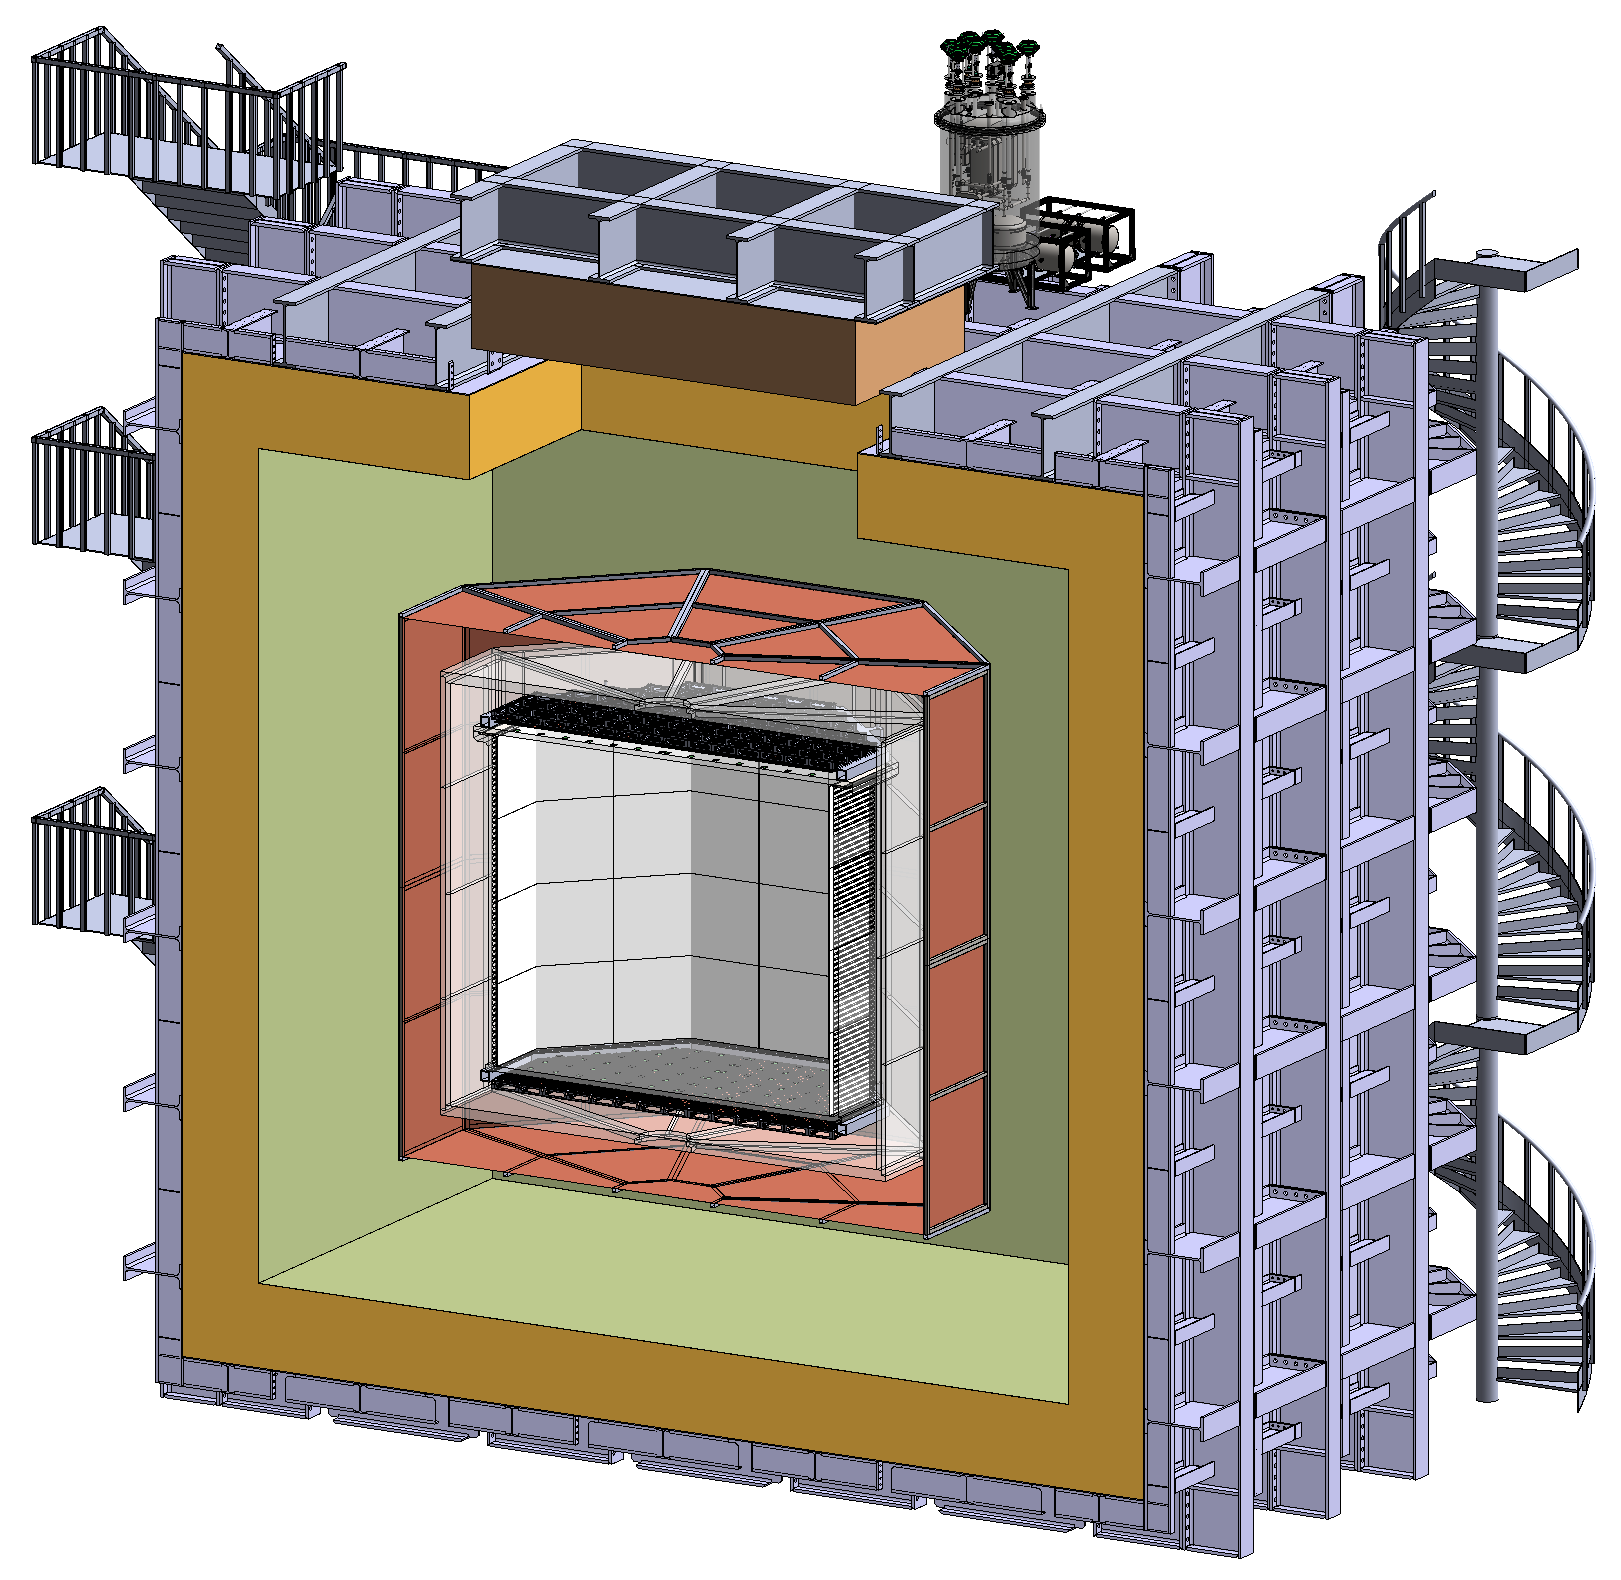
\includegraphics[width=\textwidth]{darkside20k}}
    
    \caption{\label{fig:darkside20k} Schematic cross section of DarkSide20k.
    From \cite[2]{aalseth2019}. The innermost cylinder is the TPC, wrapped in
    the two layers of the veto detector. The outer container is the cryostat,
    copied from the ProtoDune experiment.}
    
\end{figure}

The outermost tank is the cryostat, which is completely filled with LAr. In
this design the argon circuit of the TPC is separate, because it is filled with
argon extracted underground (UAr) and purified to have about 1/1400 the amount
of radioactive $^{39}$Ar isotope relative to argon distilled from the
atmosphere (AAr), which is used instead for the rest of the system.

At the top of the TPC vessel, just below the photodetectors, a ``pocket''
facing downward, like a diving bell, is kept filled with gaseous argon. An
additional grid provides an higher electric field in the gaseous phase, called
``extraction field''. When the electrons emerge from the liquid phase, they are
accelerated toward the anode and produce scintillation in the argon vapor. This
process is called electroluminescence, or secondary scintillation. The
extraction field is not intense enough to induce further ionization when the
electrons pass, so the information on the number of ionized electrons is
preserved. Most of this light hits the top photodetection plane concentrated in
a narrow spot.

The prompt photons produced by the recoil are called S1, while the light
emitted by extracted electrons S2. The names stand for ``first signal'' and
``second signal'', since S2 arrives after S1 due to the drift time. This delay
allows to deduce the depth of the recoil, i.e., the $z$ coordinate. Since most
of the S2 light is concentrated, it is easy to measure its position on the
horizontal photodetector plane. The electrons drift vertically, with little
transverse diffusion, so the reconstructed $xy$ S2 position matches the $xy$
coordinates of the recoil. Thus the TPC permits a 3D reconstruction of the
signals.

\section{Photodetectors}

DarkSide-50 uses photomultiplier tubes (PMTs) for photodetection. DarkSide20k
instead will be equipped with silicon photomultipliers (SiPMs). The SiPMs are
large matrices of photodiodes connected in parallel and operated in Geiger
mode. The advantages of SiPMs compared to PMTs are:
%
\begin{itemize}
    
    \item better single photon resolution;
    
    \item higher filling factor, i.e., they tile more densely the surface;
    
    \item low bias voltage;
    
    \item better radio-purity;
    
    \item higher photon detection efficiency (PDE).

\end{itemize}

The basic unit of the photodetection system is the photodetector module (PDM),
consisting of a Tile, i.e., a $6\times 4$ matrix of SiPMs totaling
\SI{25}{cm^2}, connected to a front end board (FEB) hosting the biasing circuit
and the preamplifier. Matrices of $5\times 5$ PDMs are bound together to form a
motherboard (MB). Each motherboard is paired with a ``steering module''
controlling the PDMs and transmission electronics, forming a photodetector unit
(PDU). \autoref{fig:sipm} shows a Tile, a FEB, a PDM and a MB.

\begin{figure}
    
    \newlength\sipmheight
    \setlength\sipmheight{5cm}
    
    \widecenter{
        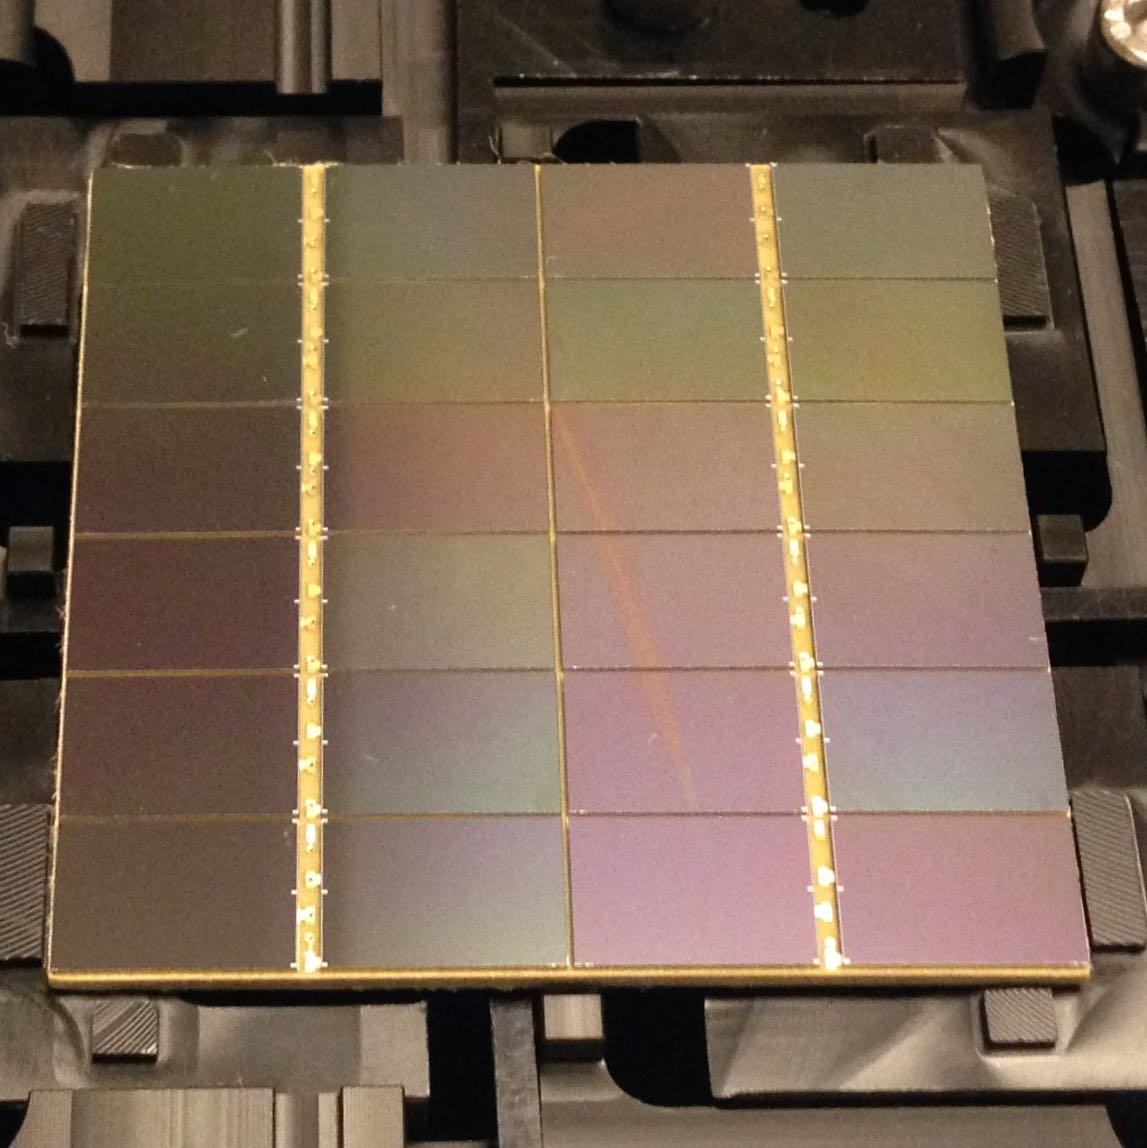
\includegraphics[height=\sipmheight]{tile}
        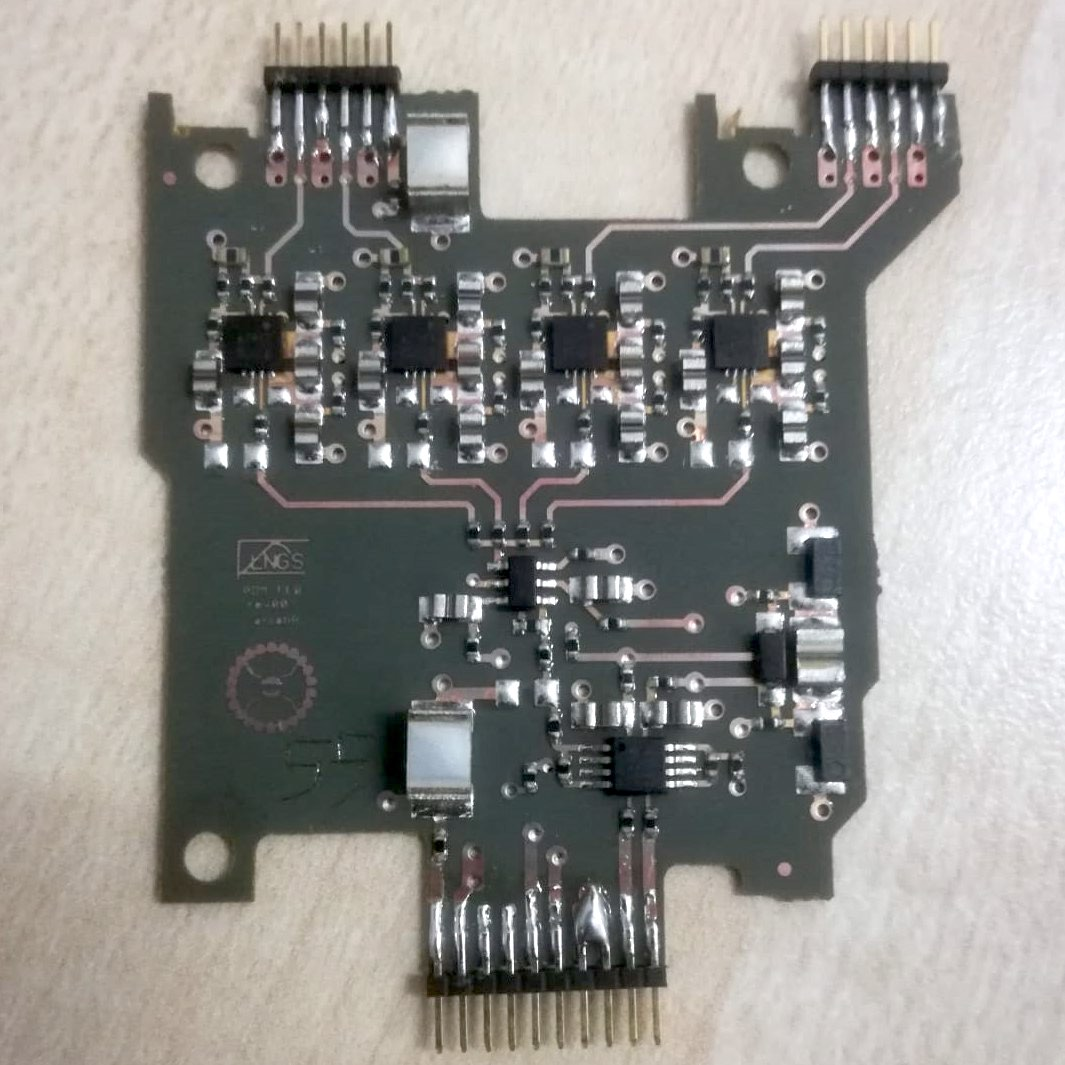
\includegraphics[height=\sipmheight]{feb}
    }

    \vspace*{1ex}
    \widecenter{
        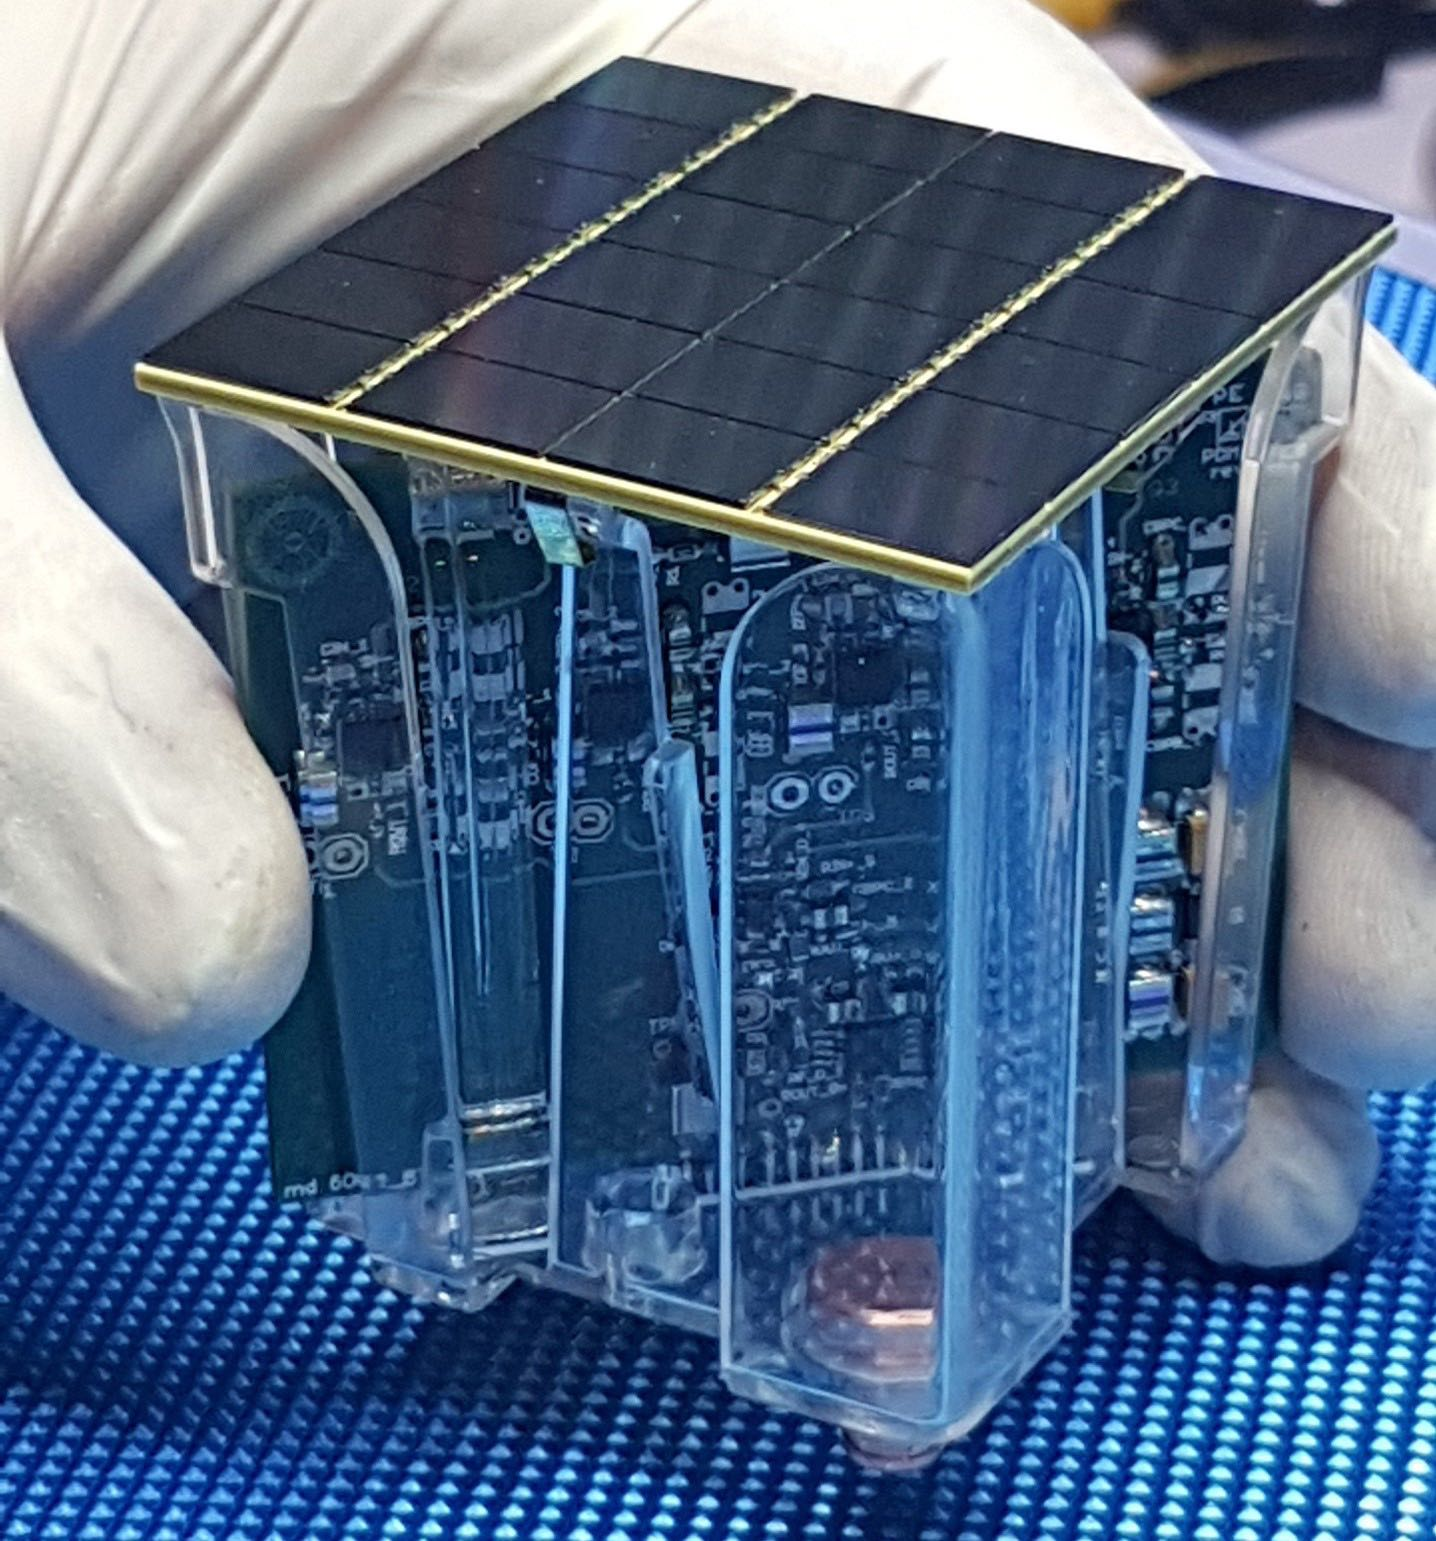
\includegraphics[height=\sipmheight]{sipm1}
        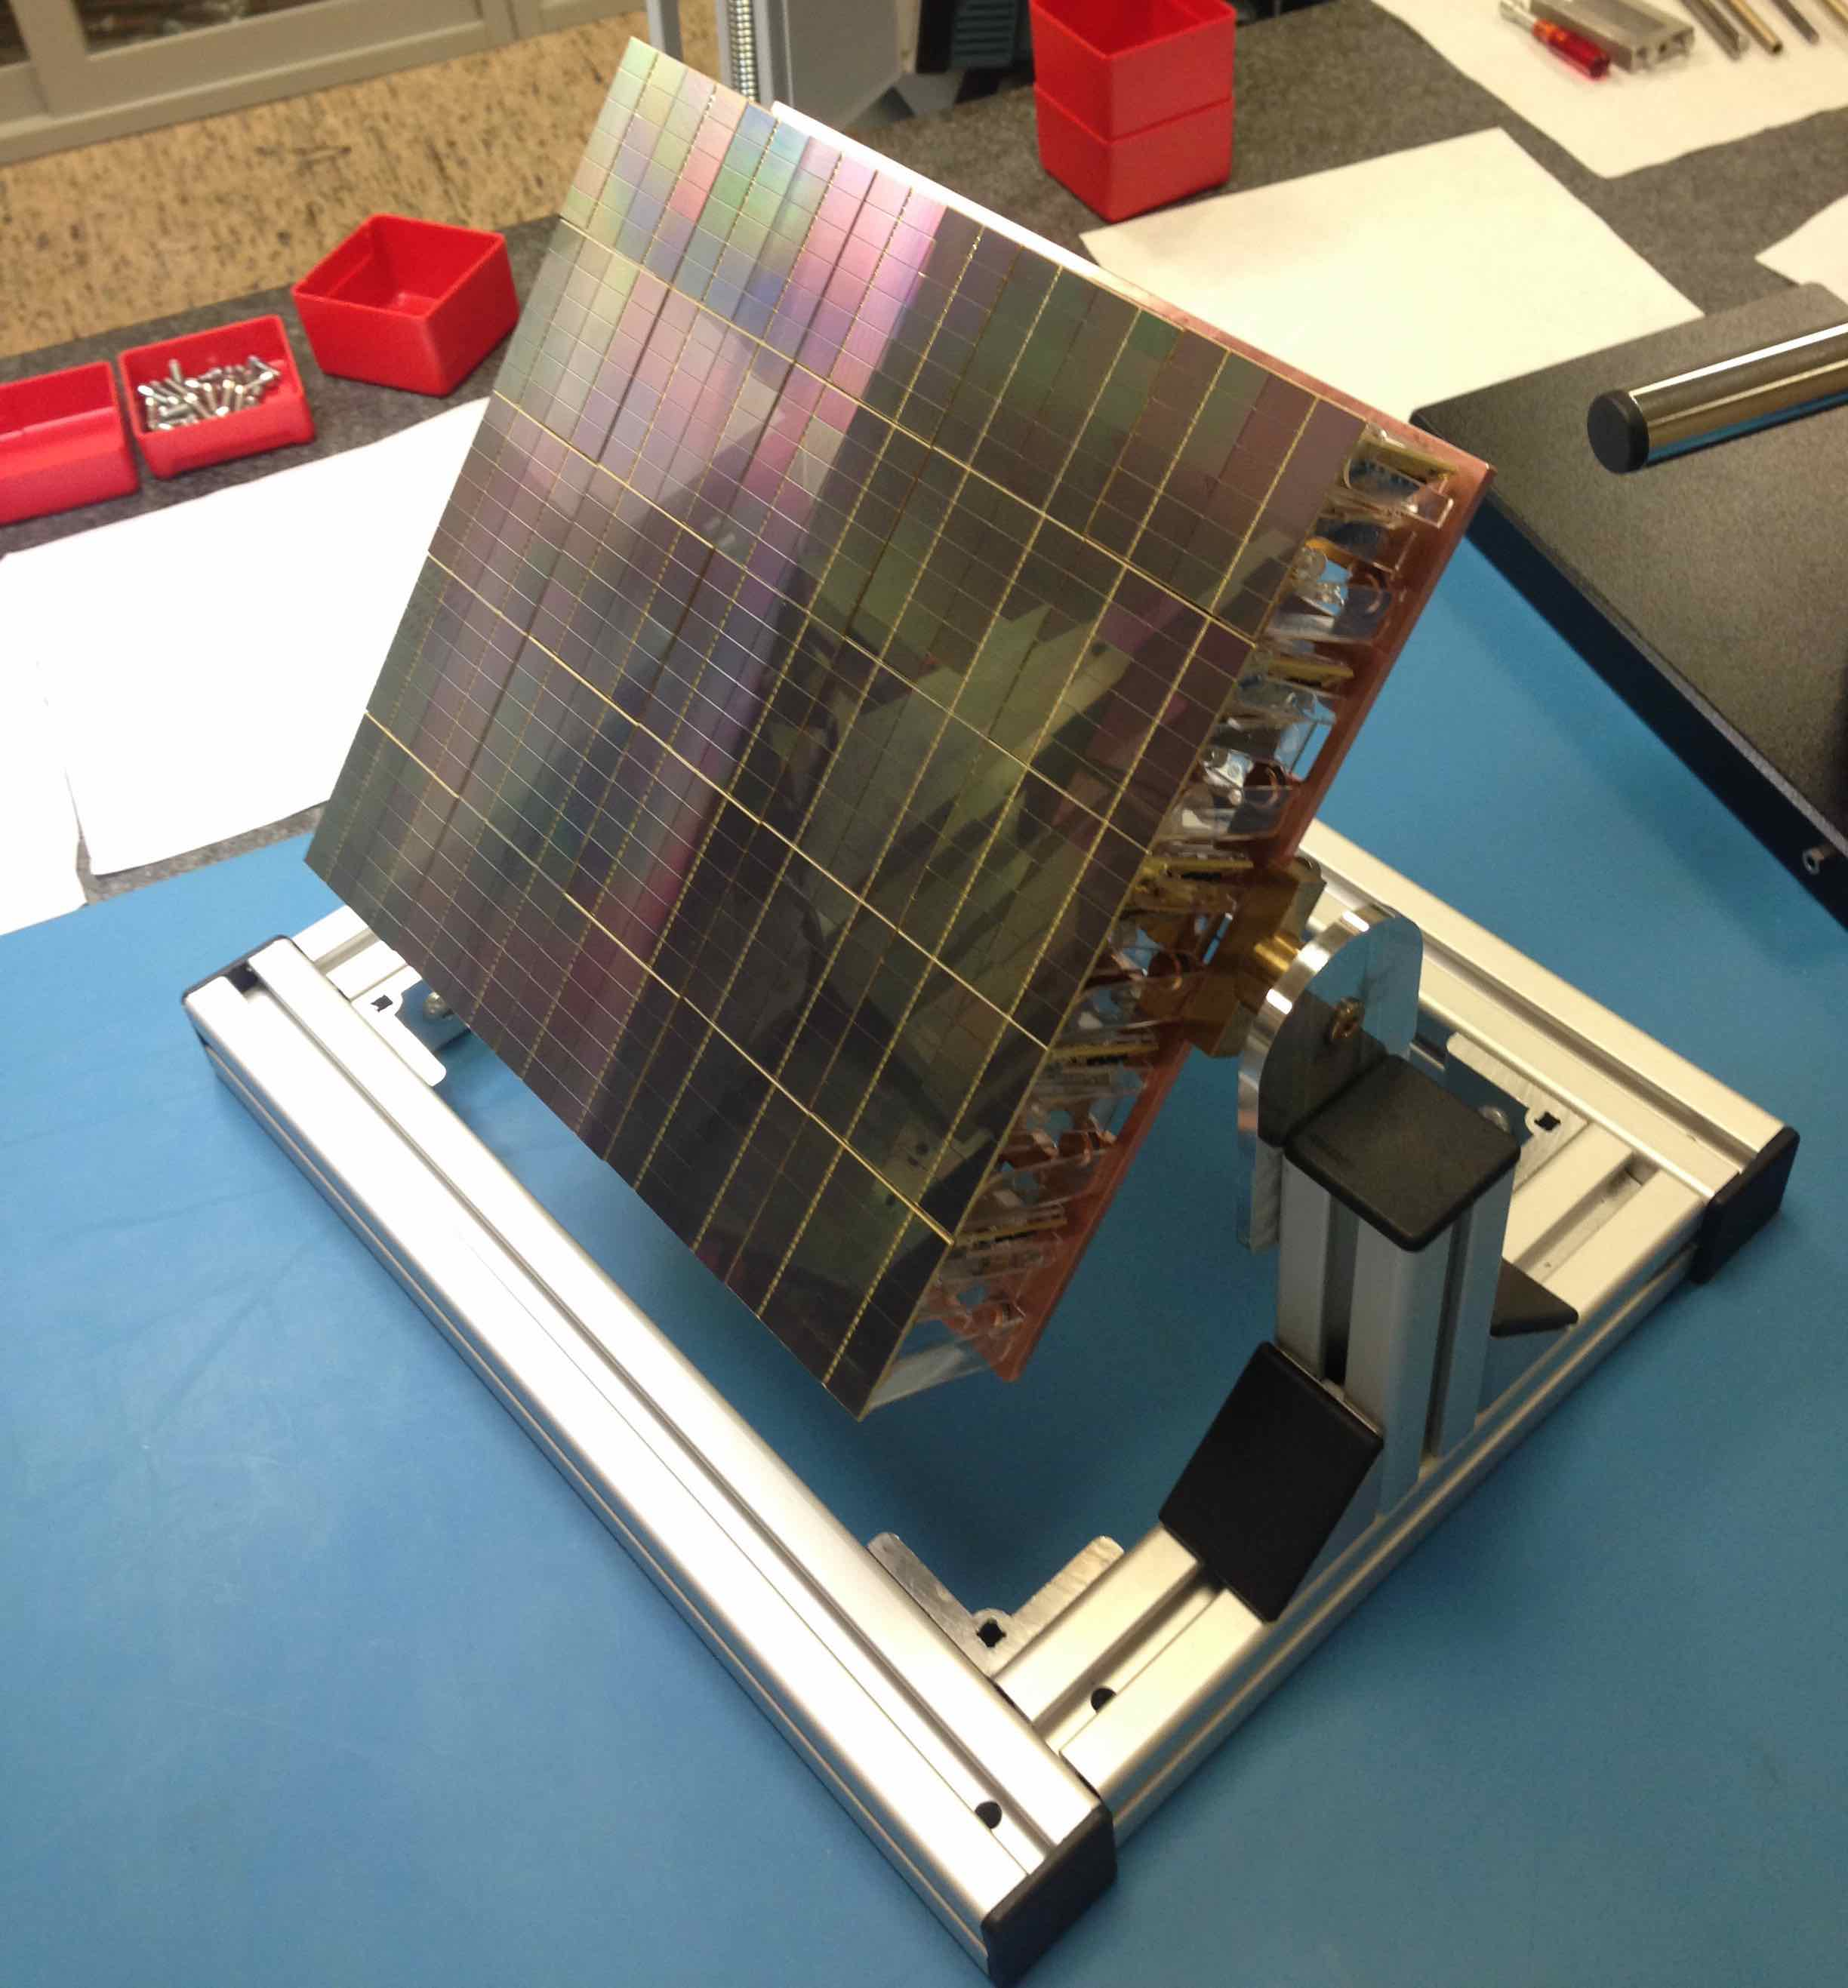
\includegraphics[height=\sipmheight]{sipm2}
    }
    
    \caption{\label{fig:sipm} Top row, left panel: a Tile, and right panel: a
    FEB, from \cite[42]{marasciulli2019}. Bottom row, left panel: a
    photodetector module (PDM), i.e., a Tile attached to a FEB, and right
    panel: a motherboard with 25 PDMs, from \cite[4]{aalseth2019}.}
    
\end{figure}

\marginpar{Da qualche parte devo definire l'overvoltage}

The Tiles are wired as follows. There are four $3\times 2$ SiPMs quadrants,
visible in \autoref{fig:sipm}. In each quadrant, SiPMs are connected in series
in pairs, and then the three branches in parallel. The quadrants are then
connected to the FEB. For each quadrant there is a trans-impedance amplifier
(TIA), which converts the current signal to a voltage signal. The outputs of
the TIAs are summed analogically. The choice of grouping multiple SiPMs in a
PDM is made to limit the number of channels to read out, for reasons of cost,
complexity, and limitation of the radiation contamination from electronic
components. The division in quadrants with separate preamplifiers, instead of a
single parallel connection, is made to reduce the input capacitance seen by the
TIAs. Electrical noise limits the number of SiPMs that can be summed
analogically into a single channel, and thus the size of the PDM.

The signals will be carried out of the cryostat to digitizer boards equipped
with 14~bit \SI{125}{MSa/s} ADCs connected to an FPGA and a controller CPU. The
digitizer board is expected to implement basic single photon pulse
identification and send selected data through an ethernet link to a front end
processor (FEP), a normal CPU station, that refines the analysis. Finally, an
event builder farm will take the information from all the FEPs, organize the
sets of photon hits into events, and decide what to record to permanent
storage.

The readout of SiPMs presents some additional issues relative to PMTs. Each
SiPM is a matrix of photodiodes connected in parallel. Since in the PDMs the
SiPMs are either connected together or summed, we can treat approximatively the
whole PDM as a single large SiPM. The random electrical noise is summed in
quadrature, so it is proportional to the square root of the area. This means
that the noise is quite high for the DarkSide20k PDMs. In practice, as we will
see in \autoref{ch:snr}, the noise RMS is comparable to the amplitude of the
single photon signals. Another issue is correlated noise. Each SiPM output
current pulse can produce other pulses, recursively, either delayed from the
parent pulse or stacked. The production of correlated noise is stochastic,
i.e., the number of additional pulses for each primary pulse fluctuates. This
implies that the extension of the dynamic range can not be compensated by
tuning the gain, and that the loss of photon count resolution is substantial.

The SiPM photodiodes are reverse biased below breakdown voltage. The production
of free carriers by an incident photon starts an avalanche, regulated with
passive quenching. The amplitude of the resulting current pulse is
approximately proportional to the difference between the bias and the breakdown
voltage, called \emph{overvoltage}. The electrical noise, instead, depends
weakly on the overvoltage, thus its effect can be mitigated by increasing the
overvoltage. However, this also increases correlated noise, because an higher
electric field in the junctions facilitates the production of charge carriers.
This means that the overvoltage is a critical parameter that must be tuned to
operate the SiPM. We defer a more complete description of the SiPM to
\autoref{ch:anal}.
